\documentclass[12pt]{article}
\title{Theory of Computation \\ Assignment 6: SAT Encoding}
\author{Brites Marto Andrea \ \ Le Thuong \\ Rodolfo Masera Tommaso \ \ Taillefert Stefano}
\date{}

\usepackage[margin=2cm]{geometry}
\usepackage{amsmath}
\usepackage[hidelinks]{hyperref}
\usepackage{amssymb}
\usepackage{caption}
\usepackage{subcaption}
\usepackage{graphicx}
\usepackage{float}


\newcommand{\mygather}[1]{\begin{gather*} #1 \end{gather*}}

\setlength{\parindent}{0cm}

\begin{document}
\maketitle

\section{Installation and Instructions}

We kindly ask you to refer to the \texttt{README.md} file that we will have attached to the assignment submission in order to install the needed dependencies and run our application properly.

As a reminder, we will also put the instructions directly in this PDF document.

First of all, you will find a text file named \texttt{requirements.txt} that contains the Python dependencies to be installed in order to run the application. You can simply run on your console:\\

\begin{center}
	\texttt{pip install --no-cache-dir -r requirements.txt}\\
	\begin{small}
		\textbf{Note:} if the command \texttt{pip} should not work, \texttt{pip3} might work instead.
	\end{small}
\end{center}

Then, if you'd like to run the program from CLI, you can simply do as follows:

\begin{center}
	\texttt{python main.py input\_file}\\

	where ``\texttt{input\_file}'' is a text file with the pairs of garments and colours $\langle g, c \rangle$. See under ``\texttt{examples/}'' or below for proper formatting.
\end{center}

If you instead would prefer to run the web server and the web application we developed, refer to these instructions:

\begin{center}
	From console: \\
	\texttt{cd app}\\
	\texttt{flask run}\\
	Head to \texttt{localhost:5000} from your browser to access the interface.\\
	If you'd like to run it with Docker, you can run \texttt{docker-compose up} from your terminal instead.
\end{center}

For an example of what an input file should look like, refer to what follows here:

A text file in the following format where the first line \texttt{garment, color} should \textbf{NOT} be changed and should \textbf{ALWAYS} be present to then follow with the pairs you would like to feed to the script. Here is an example:

\begin{center}

	{
		\ttfamily
		garment, color\\
		shirt, black\\
		shorts, white\\
		jacket, blue\\
}
\end{center}

\section{Problem Design and Interpretation}\label{section:design}

    First and foremost this problem is very loosely defined, which means that it was mostly up to us to come up with constraints or with an appropriate problem size. Our input is a pair of garments and colours $\langle g, c \rangle$, where $g \in G$ and $c \in C$; $G$ and $C$ are sets that include garments and colours respectively, both of size $10$, and are defined as follows:

    \mygather{
        G = \{\text{pants, shirt, hat, jacket, sweater, gloves, shoes, tie, scarf, shorts} \} \\
        S = \{\text{red, yellow, orange, green, blue, purple, brown, pink, white, black} \}
    }

    We chose a small size for the sake of simplicity of the project and for a more realistic aspect. We will go over this part in more detail in \textbf{section \ref{section:issues}}.

    Given these two sets, we devised constraints over them that will always be added. They are hardcoded as they specify, for instance, which garments (or colours) should or should not go together.
    We define these constraints as follows in a boolean way:

    \begin{center}
    \begin{tabular}{|l|}
    \hline
    Boolean Constraints \\
    \hline
    $\neg$(yellow $\wedge$ white) \\[0.1cm]
    $\neg$(blue $\wedge$ purple) \\[0.1cm]
    $\neg$(blue $\wedge$ black) \\[0.1cm]
    $\neg$(red $\wedge$ green) \\[0.1cm]
    $\neg$(red $\wedge$ orange) \\[0.1cm]
    $\neg$(green $\wedge$ pink) \\[0.1cm]
    $\neg$(green $\wedge$ orange) \\[0.1cm]
    $\neg$(pants $\wedge$ shorts) \\[0.1cm]
    $\neg$(shorts $\wedge$ jacket) \\[0.1cm]
    scarf $\rightarrow$ jacket \\[0.1cm]
    gloves $\rightarrow$ jacket \\[0.1cm]
    tie $\rightarrow$ shirt \\
    \hline
    \end{tabular}
    \end{center}

    Finally, we go over the given input file and we determine the final constraints. If one of the garments is missing, we make sure that they are put in a \textbf{NOT} boolean operator to take their absence into account; otherwise, if present, we simply add to our constraints list an \textbf{OR} operator of an \textbf{AND} over a pair comprising a garment $g$ and its color $c$. So basically, over an input $\langle g, c \rangle$, we would either obtain $\neg g$ if absent or $(g \wedge c)$ otherwise.


\section{Implementation}

    \subsection{SAT Solver}
        The main core of the project is the solver program (\texttt{main.py}), written entirely in Python 3. 
        We used the \texttt{z3-solver} library (\url{https://github.com/Z3Prover/z3}) to get most of the job done since it provided us with the functionalities
        we needed and was very straightforward to use. We also used \texttt{pandas} to read the input file. No, we did not ask a bunch of fluffy animals to read out the text, it's a Python library. Come on.\\
        Our program first puts the input pairs of garments and colors into a set, to filter out duplicates. Then, we build the constraints list as detailed in section \ref{section:design} and we check whether the model is
        satisfiable or not. If it's the case, we print out the solution.

    \subsection{User Interface}
        We needed to quickly develop a solid interface; the perfect candidate for this, given our skills, was a webpage. Therefore, given that the rest of the code
        was already in Python, we resorted to \texttt{Flask}, which is a simple yet powerful library to make web applications.\\
        The script (\texttt{app/app.py}) simply renders an HTML page with two inputs to compose the mannequin and a canvas to represent the solution, which is obtained by 
        calling our solver with the given input data.

        \begin{figure}[H]
            \centering
            \begin{subfigure}{0.49\textwidth}
                    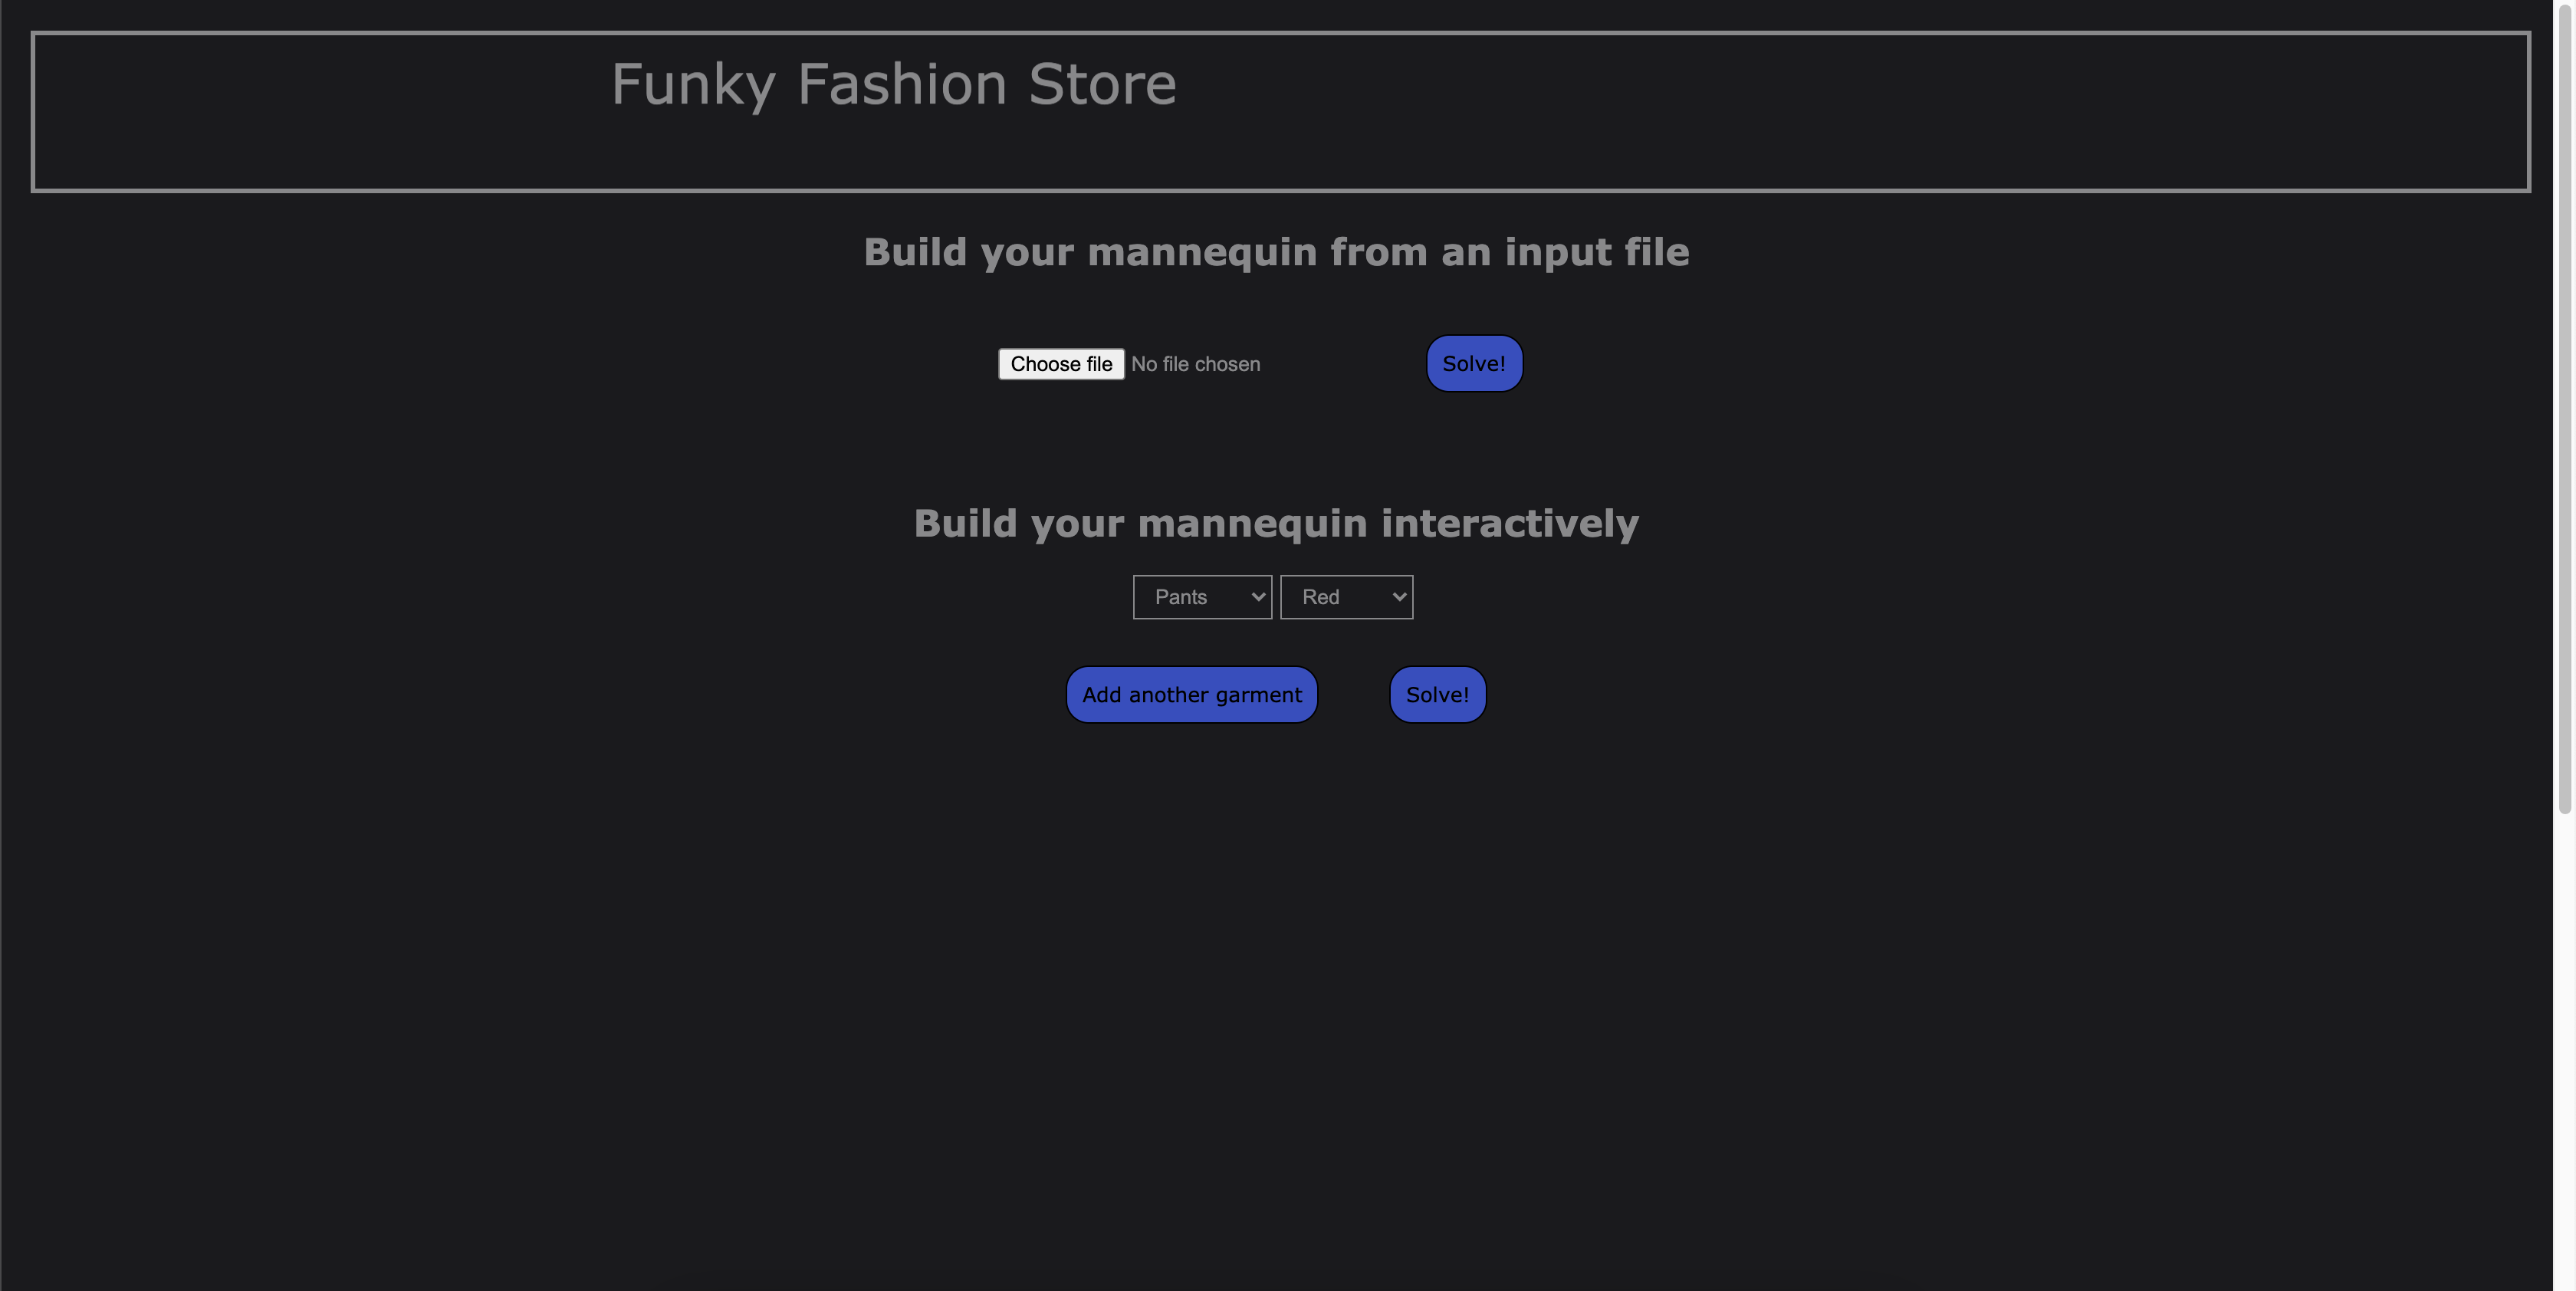
\includegraphics[width=\textwidth]{img/interface1.png}
                    \caption{The homepage}
            \end{subfigure}
            \begin{subfigure}{0.49\textwidth}
                    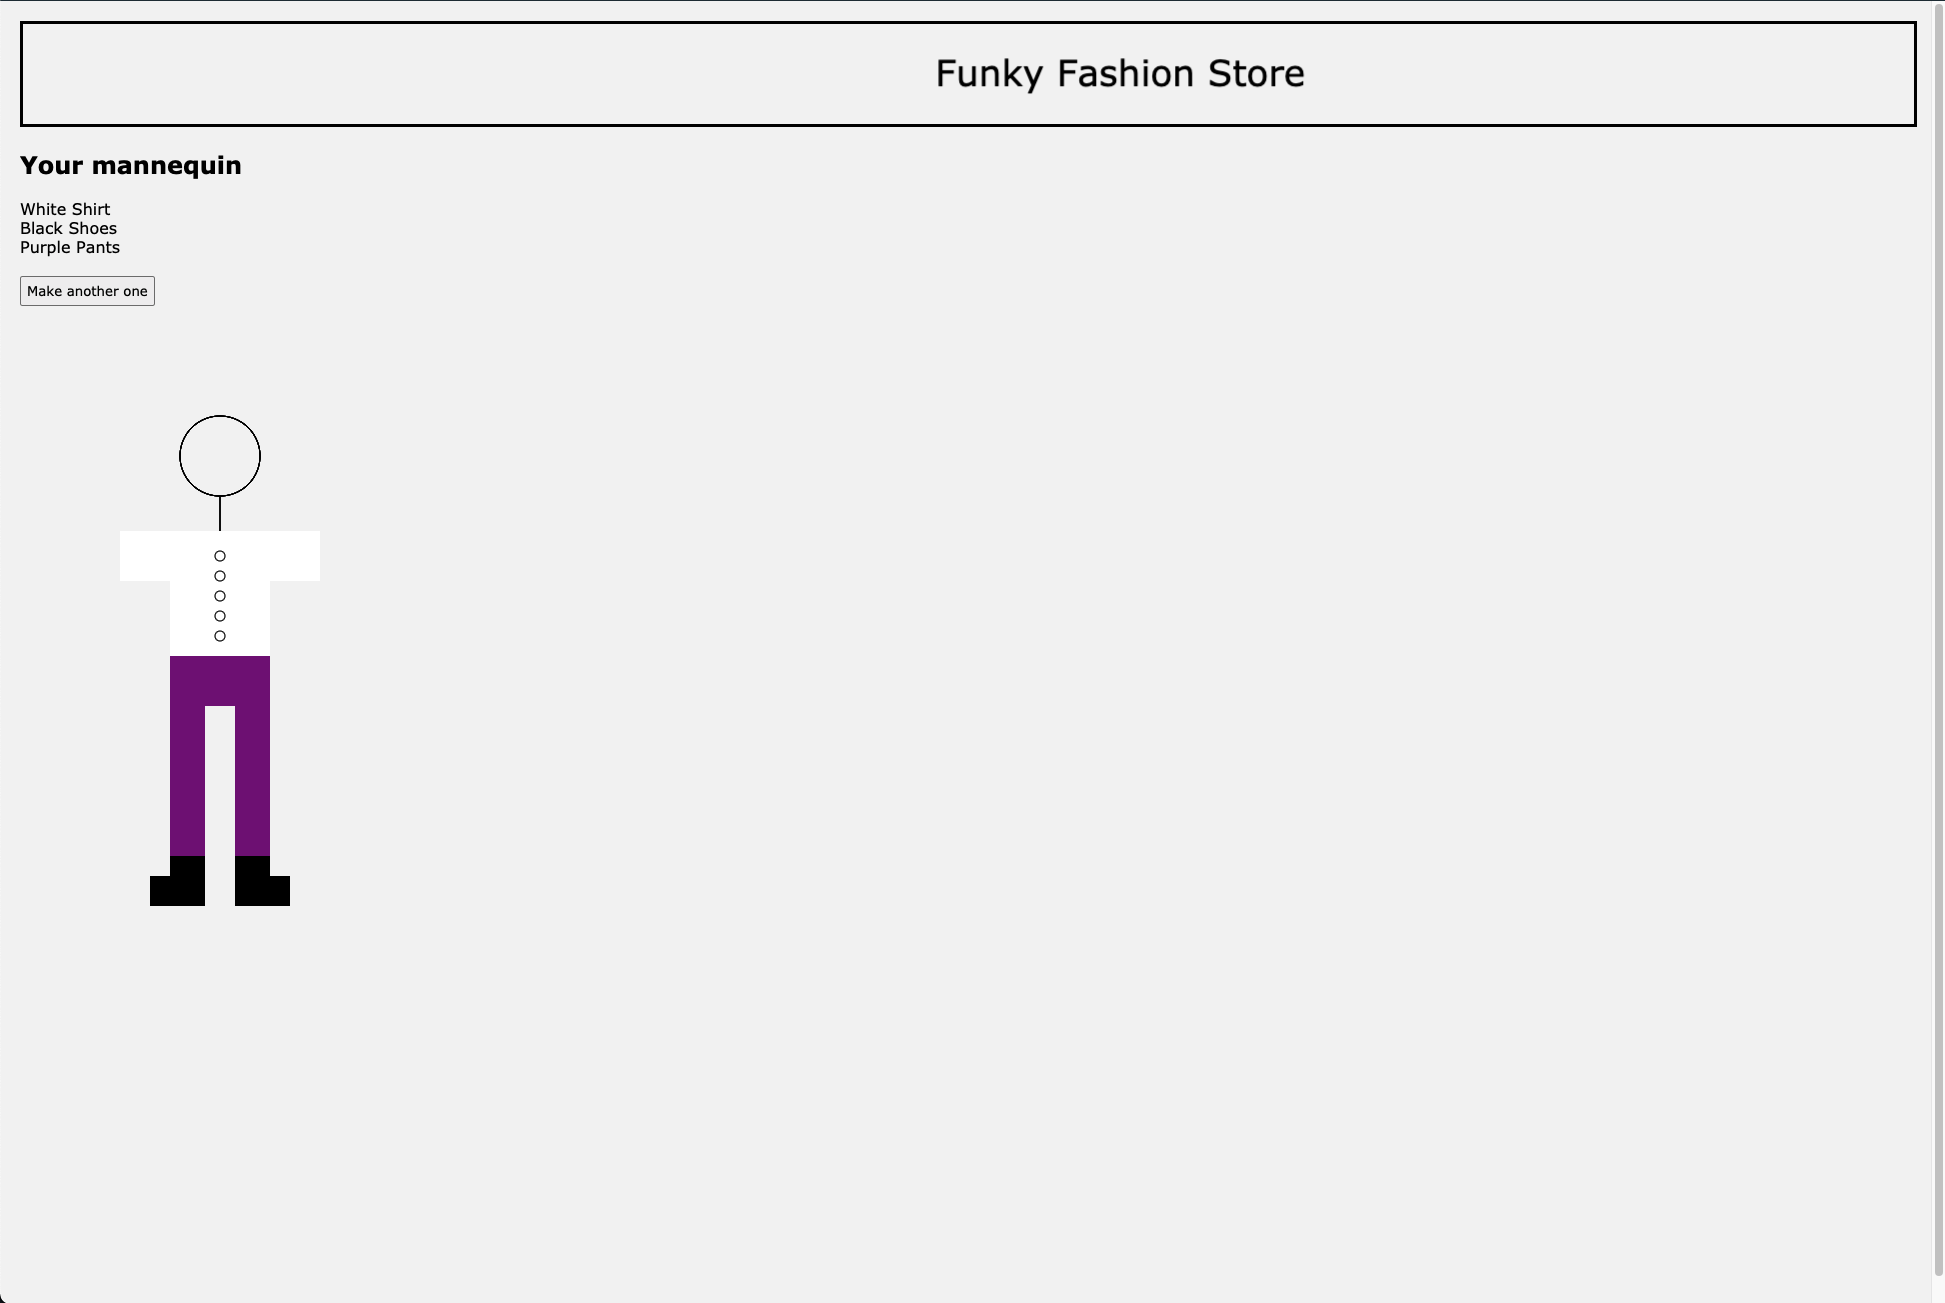
\includegraphics[width=\textwidth]{img/interface2.png}
                    \caption{A solved mannequin}
            \end{subfigure}
        \end{figure}

    \subsection{Deployment}
        Since we built a web interface, we thought it would be a good idea to deploy our project as a fully functional website. 
        For this reason, we purchased the domain \url{bestsatsolver.xyz}, packed our app in a Docker container and put it on a small server of ours.
        The whole process was pretty straightforward, given that our project has a very simple structure and doesn't depend on other services like databases or external APIs.

\section{Issues Encountered}
\label{section:issues}

Other than the typical issues that may arise when programming (i.e. bugs, code design, ...), the main issue that we encountered ended up being caused by the fact that the problem assigned to us was loosely defined. This meant that we had freedom to pick on how to develop it but that we also had to make sure to keep it complete while not overcomplicating it.\\

As we had described in \textbf{section \ref{section:design}}, we decided to keep the size of the problem relatively small by limiting the possible colors and garments to a set of ten elements each. Along with the fact that, in reality, oftentimes we would not expect to have to dress a mannequin with thousands of garments and colours, we also thought that it would be easier to define our own sets and constraints over them rather than to allow variable input sizes.\\

The main issue that would have come with a variable input size where you would allow the input to decide how many garments and colours would be available (along with the subsequent possible pairs) would have been to define the constraints over the sets of colours and garments.\\

For instance, if we take our own sets, we have ten garments and ten colours and we have added constraints with the knowledge of those garments and colours.

If for example we had $x$ garments and $y$ colours where $x, y \in \mathbb{N}$, we then would first of all have $x \cdot y$ possible pairs and, furthermore, defining the constraints over them would be incredibly tough and we might have to take a randomized approach: given $x$ garments and $y$ colours and a set $S$ containing a pair of garments and colours $\langle g, c \rangle$, we take a random garment $g$ and we put a constraint over it with respect to another garment $g'$, same approach for the colours.\\

Therefore, given the fact that a variable input size with respect to the number of garments and colours would be tougher to work with, we have delimited the problem to two given sets of size ten each where we can clearly define our constraints.


\end{document}
